\documentclass[tikz=true]{standalone}
\begin{document}
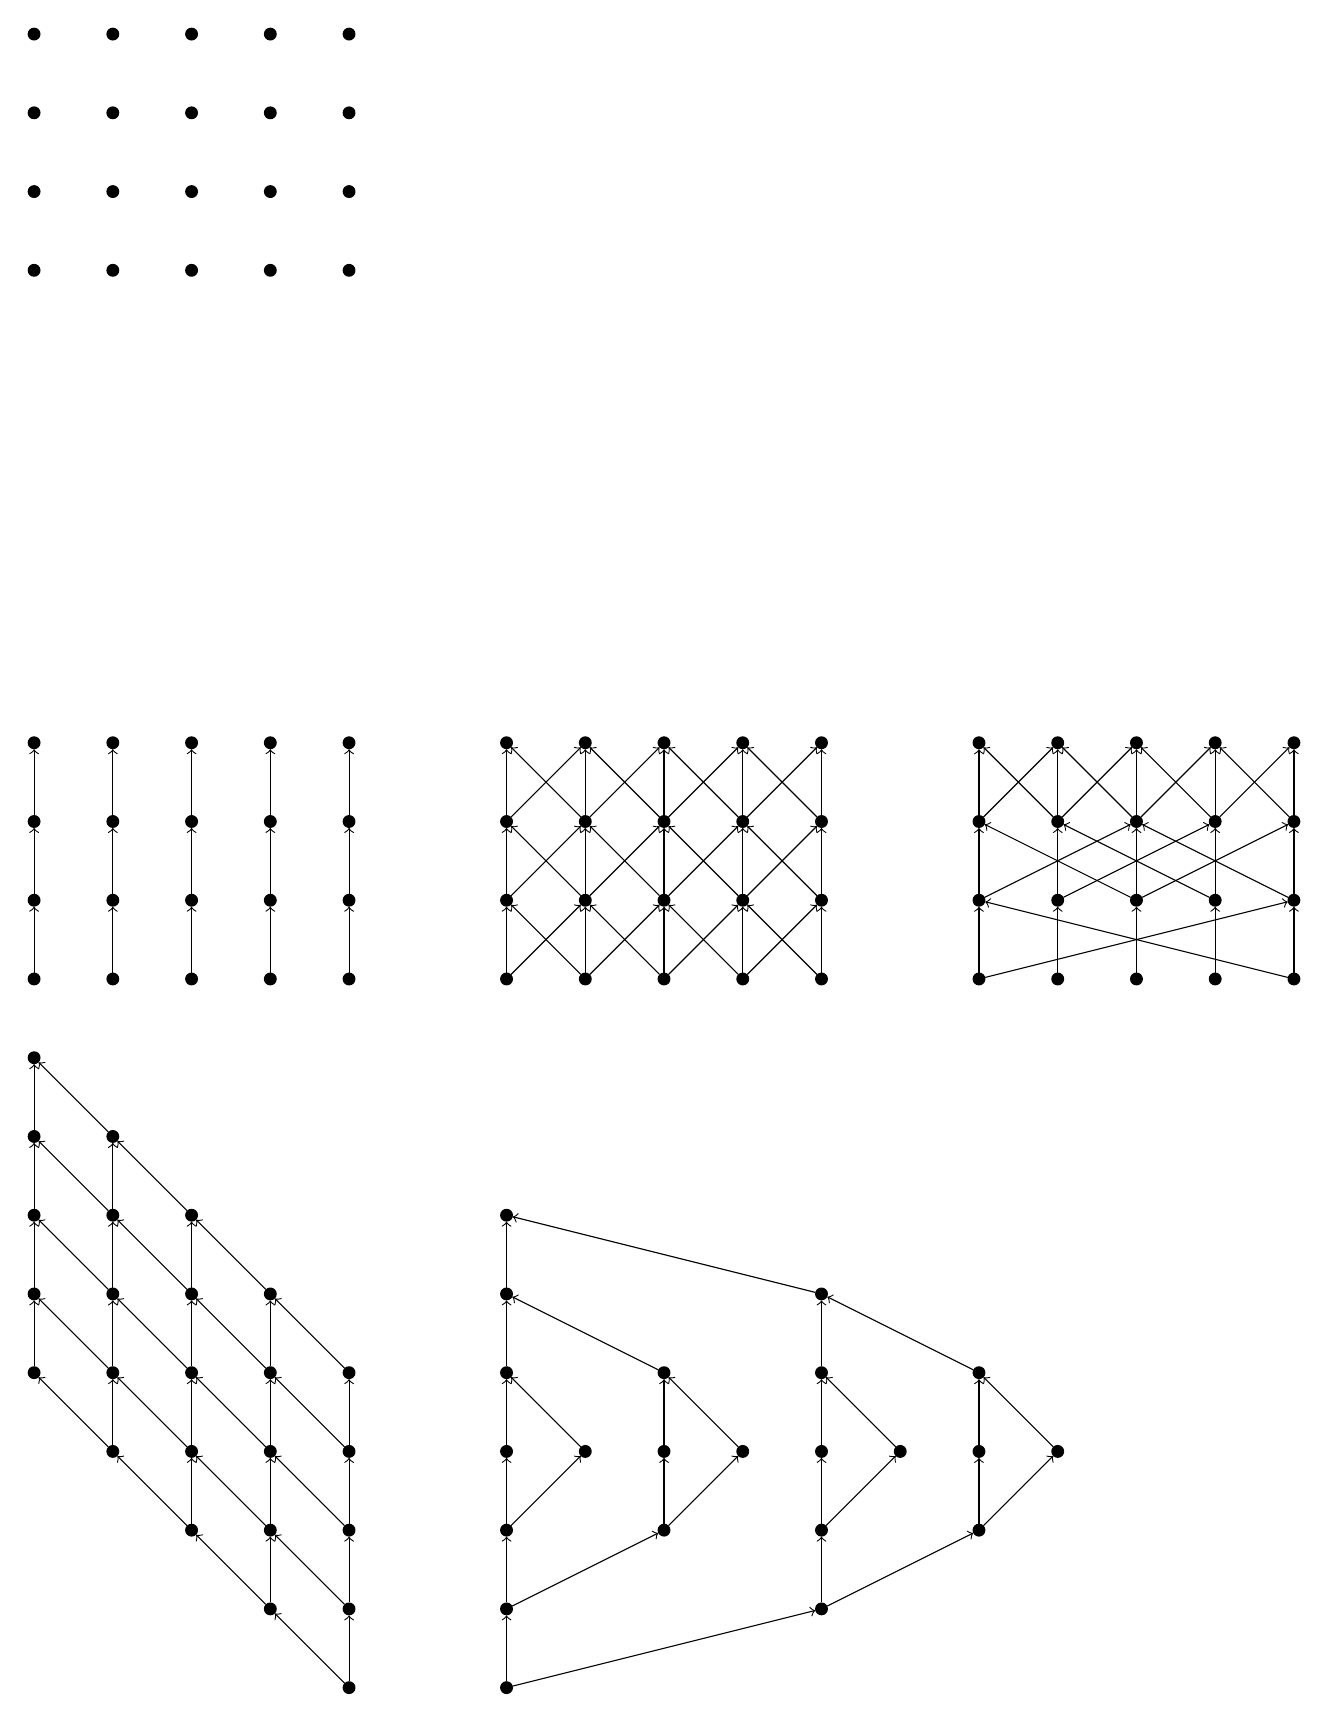
\begin{tikzpicture}
  % Trivial
  \begin{scope}[every node/.style={draw, shape=circle, fill=black, inner sep=1.5pt, shift={(0,9)}}]
    \node (n00) at (0,0) {};
    \node (n01) at (0,1) {};
    \node (n02) at (0,2) {};
    \node (n03) at (0,3) {};

    \node (n10) at (1,0) {};
    \node (n11) at (1,1) {};
    \node (n12) at (1,2) {};
    \node (n13) at (1,3) {};

    \node (n20) at (2,0) {};
    \node (n21) at (2,1) {};
    \node (n22) at (2,2) {};
    \node (n23) at (2,3) {};

    \node (n30) at (3,0) {};
    \node (n31) at (3,1) {};
    \node (n32) at (3,2) {};
    \node (n33) at (3,3) {};

    \node (n40) at (4,0) {};
    \node (n41) at (4,1) {};
    \node (n42) at (4,2) {};
    \node (n43) at (4,3) {};
  \end{scope}

  % No Comm
  \begin{scope}[every node/.style={draw, shape=circle, fill=black, inner sep=1.5pt, shift={(0,0)}}]
    \node (n00) at (0,0) {};
    \node (n01) at (0,1) {};
    \node (n02) at (0,2) {};
    \node (n03) at (0,3) {};

    \node (n10) at (1,0) {};
    \node (n11) at (1,1) {};
    \node (n12) at (1,2) {};
    \node (n13) at (1,3) {};

    \node (n20) at (2,0) {};
    \node (n21) at (2,1) {};
    \node (n22) at (2,2) {};
    \node (n23) at (2,3) {};

    \node (n30) at (3,0) {};
    \node (n31) at (3,1) {};
    \node (n32) at (3,2) {};
    \node (n33) at (3,3) {};

    \node (n40) at (4,0) {};
    \node (n41) at (4,1) {};
    \node (n42) at (4,2) {};
    \node (n43) at (4,3) {};

    % Straight
    \draw[->] (n00) edge (n01);
    \draw[->] (n01) edge (n02);
    \draw[->] (n02) edge (n03);

    \draw[->] (n10) edge (n11);
    \draw[->] (n11) edge (n12);
    \draw[->] (n12) edge (n13);

    \draw[->] (n20) edge (n21);
    \draw[->] (n21) edge (n22);
    \draw[->] (n22) edge (n23);

    \draw[->] (n30) edge (n31);
    \draw[->] (n31) edge (n32);
    \draw[->] (n32) edge (n33);

    \draw[->] (n40) edge (n41);
    \draw[->] (n41) edge (n42);
    \draw[->] (n42) edge (n43);
  \end{scope}

  % Stencil
  \begin{scope}[every node/.style={draw, shape=circle, fill=black, inner sep=1.5pt, shift={(6,0)}}]
    \node (n00) at (0,0) {};
    \node (n01) at (0,1) {};
    \node (n02) at (0,2) {};
    \node (n03) at (0,3) {};

    \node (n10) at (1,0) {};
    \node (n11) at (1,1) {};
    \node (n12) at (1,2) {};
    \node (n13) at (1,3) {};

    \node (n20) at (2,0) {};
    \node (n21) at (2,1) {};
    \node (n22) at (2,2) {};
    \node (n23) at (2,3) {};

    \node (n30) at (3,0) {};
    \node (n31) at (3,1) {};
    \node (n32) at (3,2) {};
    \node (n33) at (3,3) {};

    \node (n40) at (4,0) {};
    \node (n41) at (4,1) {};
    \node (n42) at (4,2) {};
    \node (n43) at (4,3) {};

    % Straight
    \draw[->] (n00) edge (n01);
    \draw[->] (n01) edge (n02);
    \draw[->] (n02) edge (n03);

    \draw[->] (n10) edge (n11);
    \draw[->] (n11) edge (n12);
    \draw[->] (n12) edge (n13);

    \draw[->] (n20) edge (n21);
    \draw[->] (n21) edge (n22);
    \draw[->] (n22) edge (n23);

    \draw[->] (n30) edge (n31);
    \draw[->] (n31) edge (n32);
    \draw[->] (n32) edge (n33);

    \draw[->] (n40) edge (n41);
    \draw[->] (n41) edge (n42);
    \draw[->] (n42) edge (n43);

    % Crossing
    \draw[->] (n30) edge (n41);

    \draw[->] (n20) edge (n31);
    \draw[->] (n31) edge (n42);

    \draw[->] (n10) edge (n21);
    \draw[->] (n21) edge (n32);
    \draw[->] (n32) edge (n43);

    \draw[->] (n00) edge (n11);
    \draw[->] (n11) edge (n22);
    \draw[->] (n22) edge (n33);

    \draw[->] (n01) edge (n12);
    \draw[->] (n12) edge (n23);

    \draw[->] (n02) edge (n13);

    \draw[->] (n10) edge (n01);

    \draw[->] (n20) edge (n11);
    \draw[->] (n11) edge (n02);

    \draw[->] (n30) edge (n21);
    \draw[->] (n21) edge (n12);
    \draw[->] (n12) edge (n03);

    \draw[->] (n40) edge (n31);
    \draw[->] (n31) edge (n22);
    \draw[->] (n22) edge (n13);

    \draw[->] (n41) edge (n32);
    \draw[->] (n32) edge (n23);

    \draw[->] (n42) edge (n33);
  \end{scope}

  % FFT
  \begin{scope}[every node/.style={draw, shape=circle, fill=black, inner sep=1.5pt, shift={(12,0)}}]
    \node (n00) at (0,0) {};
    \node (n01) at (0,1) {};
    \node (n02) at (0,2) {};
    \node (n03) at (0,3) {};

    \node (n10) at (1,0) {};
    \node (n11) at (1,1) {};
    \node (n12) at (1,2) {};
    \node (n13) at (1,3) {};

    \node (n20) at (2,0) {};
    \node (n21) at (2,1) {};
    \node (n22) at (2,2) {};
    \node (n23) at (2,3) {};

    \node (n30) at (3,0) {};
    \node (n31) at (3,1) {};
    \node (n32) at (3,2) {};
    \node (n33) at (3,3) {};

    \node (n40) at (4,0) {};
    \node (n41) at (4,1) {};
    \node (n42) at (4,2) {};
    \node (n43) at (4,3) {};

    % Straight
    \draw[->] (n00) edge (n01);
    \draw[->] (n01) edge (n02);
    \draw[->] (n02) edge (n03);

    \draw[->] (n10) edge (n11);
    \draw[->] (n11) edge (n12);
    \draw[->] (n12) edge (n13);

    \draw[->] (n20) edge (n21);
    \draw[->] (n21) edge (n22);
    \draw[->] (n22) edge (n23);

    \draw[->] (n30) edge (n31);
    \draw[->] (n31) edge (n32);
    \draw[->] (n32) edge (n33);

    \draw[->] (n40) edge (n41);
    \draw[->] (n41) edge (n42);
    \draw[->] (n42) edge (n43);

    % Crossing
    % by 1
    \draw[->] (n32) edge (n43);
    \draw[->] (n22) edge (n33);
    \draw[->] (n12) edge (n23);
    \draw[->] (n02) edge (n13);

    \draw[->] (n12) edge (n03);
    \draw[->] (n22) edge (n13);
    \draw[->] (n32) edge (n23);
    \draw[->] (n42) edge (n33);

    % by 2
    \draw[->] (n21) edge (n42);
    \draw[->] (n11) edge (n32);
    \draw[->] (n01) edge (n22);

    \draw[->] (n21) edge (n02);
    \draw[->] (n31) edge (n12);
    \draw[->] (n41) edge (n22);

    % by 4
    \draw[->] (n00) edge (n41);

    \draw[->] (n40) edge (n01);

  \end{scope}

  % DOM
  \begin{scope}[every node/.style={draw, shape=circle, fill=black, inner sep=1.5pt, shift={(0,-9)}}]
    \node (n04) at (0,4) {};
    \node (n05) at (0,5) {};
    \node (n06) at (0,6) {};
    \node (n07) at (0,7) {};
    \node (n08) at (0,8) {};

    \node (n13) at (1,3) {};
    \node (n14) at (1,4) {};
    \node (n15) at (1,5) {};
    \node (n16) at (1,6) {};
    \node (n17) at (1,7) {};

    \node (n22) at (2,2) {};
    \node (n23) at (2,3) {};
    \node (n24) at (2,4) {};
    \node (n25) at (2,5) {};
    \node (n26) at (2,6) {};

    \node (n31) at (3,1) {};
    \node (n32) at (3,2) {};
    \node (n33) at (3,3) {};
    \node (n34) at (3,4) {};
    \node (n35) at (3,5) {};

    \node (n40) at (4,0) {};
    \node (n41) at (4,1) {};
    \node (n42) at (4,2) {};
    \node (n43) at (4,3) {};
    \node (n44) at (4,4) {};

    % Straight
    \draw[->] (n04) edge (n05);
    \draw[->] (n05) edge (n06);
    \draw[->] (n06) edge (n07);
    \draw[->] (n07) edge (n08);

    \draw[->] (n13) edge (n14);
    \draw[->] (n14) edge (n15);
    \draw[->] (n15) edge (n16);
    \draw[->] (n16) edge (n17);

    \draw[->] (n22) edge (n23);
    \draw[->] (n23) edge (n24);
    \draw[->] (n24) edge (n25);
    \draw[->] (n25) edge (n26);

    \draw[->] (n31) edge (n32);
    \draw[->] (n32) edge (n33);
    \draw[->] (n33) edge (n34);
    \draw[->] (n34) edge (n35);

    \draw[->] (n40) edge (n41);
    \draw[->] (n41) edge (n42);
    \draw[->] (n42) edge (n43);
    \draw[->] (n43) edge (n44);

    % Crossing
    \draw[->] (n40) edge (n31);
    \draw[->] (n31) edge (n22);
    \draw[->] (n22) edge (n13);
    \draw[->] (n13) edge (n04);

    \draw[->] (n41) edge (n32);
    \draw[->] (n32) edge (n23);
    \draw[->] (n23) edge (n14);
    \draw[->] (n14) edge (n05);

    \draw[->] (n42) edge (n33);
    \draw[->] (n33) edge (n24);
    \draw[->] (n24) edge (n15);
    \draw[->] (n15) edge (n06);

    \draw[->] (n43) edge (n34);
    \draw[->] (n34) edge (n25);
    \draw[->] (n25) edge (n16);
    \draw[->] (n16) edge (n07);

    \draw[->] (n44) edge (n35);
    \draw[->] (n35) edge (n26);
    \draw[->] (n26) edge (n17);
    \draw[->] (n17) edge (n08);
  \end{scope}


  % Tree
  \begin{scope}[every node/.style={draw, shape=circle, fill=black, inner sep=1.5pt, shift={(6,-9)}}]
    \node (n00) at (0,0) {};
    \node (n01) at (0,1) {};
    \node (n02) at (0,2) {};
    \node (n03) at (0,3) {};
    \node (n04) at (0,4) {};
    \node (n05) at (0,5) {};
    \node (n06) at (0,6) {};

    \node (n13) at (1,3) {};

    \node (n22) at (2,2) {};
    \node (n23) at (2,3) {};
    \node (n24) at (2,4) {};

    \node (n33) at (3,3) {};

    \node (n41) at (4,1) {};
    \node (n42) at (4,2) {};
    \node (n43) at (4,3) {};
    \node (n44) at (4,4) {};
    \node (n45) at (4,5) {};

    \node (n53) at (5,3) {};

    \node (n62) at (6,2) {};
    \node (n63) at (6,3) {};
    \node (n64) at (6,4) {};

    \node (n73) at (7,3) {};

    \draw[->] (n00) edge (n01);
    \draw[->] (n00) edge (n41);

    \draw[->] (n01) edge (n02);
    \draw[->] (n01) edge (n22);

    \draw[->] (n41) edge (n42);
    \draw[->] (n41) edge (n62);

    \draw[->] (n02) edge (n03);
    \draw[->] (n02) edge (n13);

    \draw[->] (n22) edge (n23);
    \draw[->] (n22) edge (n33);

    \draw[->] (n42) edge (n43);
    \draw[->] (n42) edge (n53);

    \draw[->] (n62) edge (n63);
    \draw[->] (n62) edge (n73);

    \draw[->] (n03) edge (n04);
    \draw[->] (n13) edge (n04);

    \draw[->] (n23) edge (n24);
    \draw[->] (n33) edge (n24);

    \draw[->] (n43) edge (n44);
    \draw[->] (n53) edge (n44);

    \draw[->] (n63) edge (n64);
    \draw[->] (n73) edge (n64);

    \draw[->] (n04) edge (n05);
    \draw[->] (n24) edge (n05);

    \draw[->] (n44) edge (n45);
    \draw[->] (n64) edge (n45);

    \draw[->] (n05) edge (n06);
    \draw[->] (n45) edge (n06);

  \end{scope}
\end{tikzpicture}
\end{document}
